\documentclass[11pt]{beamer}
% Packages
\usepackage{beamer-german}

% Title etc.
\title{Politische Kultur}
\subtitle{Analyse politischer Unterstützung in der quantitativen Forschungspraxis}
\date{12. November 2021}
\author{B. Philipp Kleer}
\institute{Institut für Politikwissenschaft | Justus-Liebig-Universität Gießen}

\setbeamerfont{itemize/enumerate body}{size = \small}
\setbeamerfont{itemize/enumerate subbody}{size = \footnotesize}
\setbeamerfont{itemize/enumerate subsubbody}{size = \scriptsize}

% Datumspaket
\usepackage[german]{isodate}

% Table packages
\usepackage{booktabs}
\usepackage{longtable}

% bibtex-file
\usepackage[backend=biber]{biblatex}
\addbibresource{lit-s3.bib} 

\begin{document}

\begin{frame}
	\titlepage
\end{frame}

\begin{frame}[t]{Heutige Agenda}
	\shine{Grundlagentexte}
	\begin{itemize}
		\item \cite{Almond1963}
		\item \cite{Gabriel2009}
	\end{itemize}
\end{frame}

\begin{frame}[t]{Gruppenstart}
	Wir gehen zuerst in Gruppen. Hier sollen Verständnisprobleme geklärt werden und die folgenden zwei Fragen diskutiert werden:
	
	\begin{nolist}
		\item Was unterscheidet den Begriff der Kultur bei Almond und Verba vom alltäglichen Kulturbegriff?
		\item Welche Anknüpfungspunkte sehen Sie zu Eastons Theorie?
	\end{nolist}
	
	\shine{Zeit}: 20 Minuten.
\end{frame}

\begin{frame}[t]{Politische Kultur}
	\shine{Wissenschaftliche Entwicklung}
	\begin{itemize}
		\item Institutionentheorien und Modernisierungstheorien konnten nicht Zusammenbruch in Deutschland/Italien erklären bzw. die Nicht-Stabilität in Kolonien \pause
	\end{itemize}
	
	\shine{Zusätzlicher Hintergrund}
	\begin{itemize}
		\item Kalter Krieg; Wie können (pro-)westliche Systeme stabil sein?
		\item Verknüpfung von Systemtheorie mit Umfrageforschung
	\end{itemize}
\end{frame}

\begin{frame}[t]{Politische Kultur}
	\shine{Leitende Forschungsfrage}
	\begin{itemize}
		\item Wie lässt sich Stabilität/Wandel von Regimen erklären? \pause
	\end{itemize}
	
	\shine{Annahmen / Hypothese}
	\begin{itemize}
		\item stabil, wenn politische Strukturen (Institutionen etc.) mit politischer Kultur (Einstellung der Bevölkerung) kompatibel ist
	\end{itemize}
\end{frame}

\begin{frame}{Alltagsbegriff vs. Wissenschaftsbegriff}
	\begin{figure}[ht]
		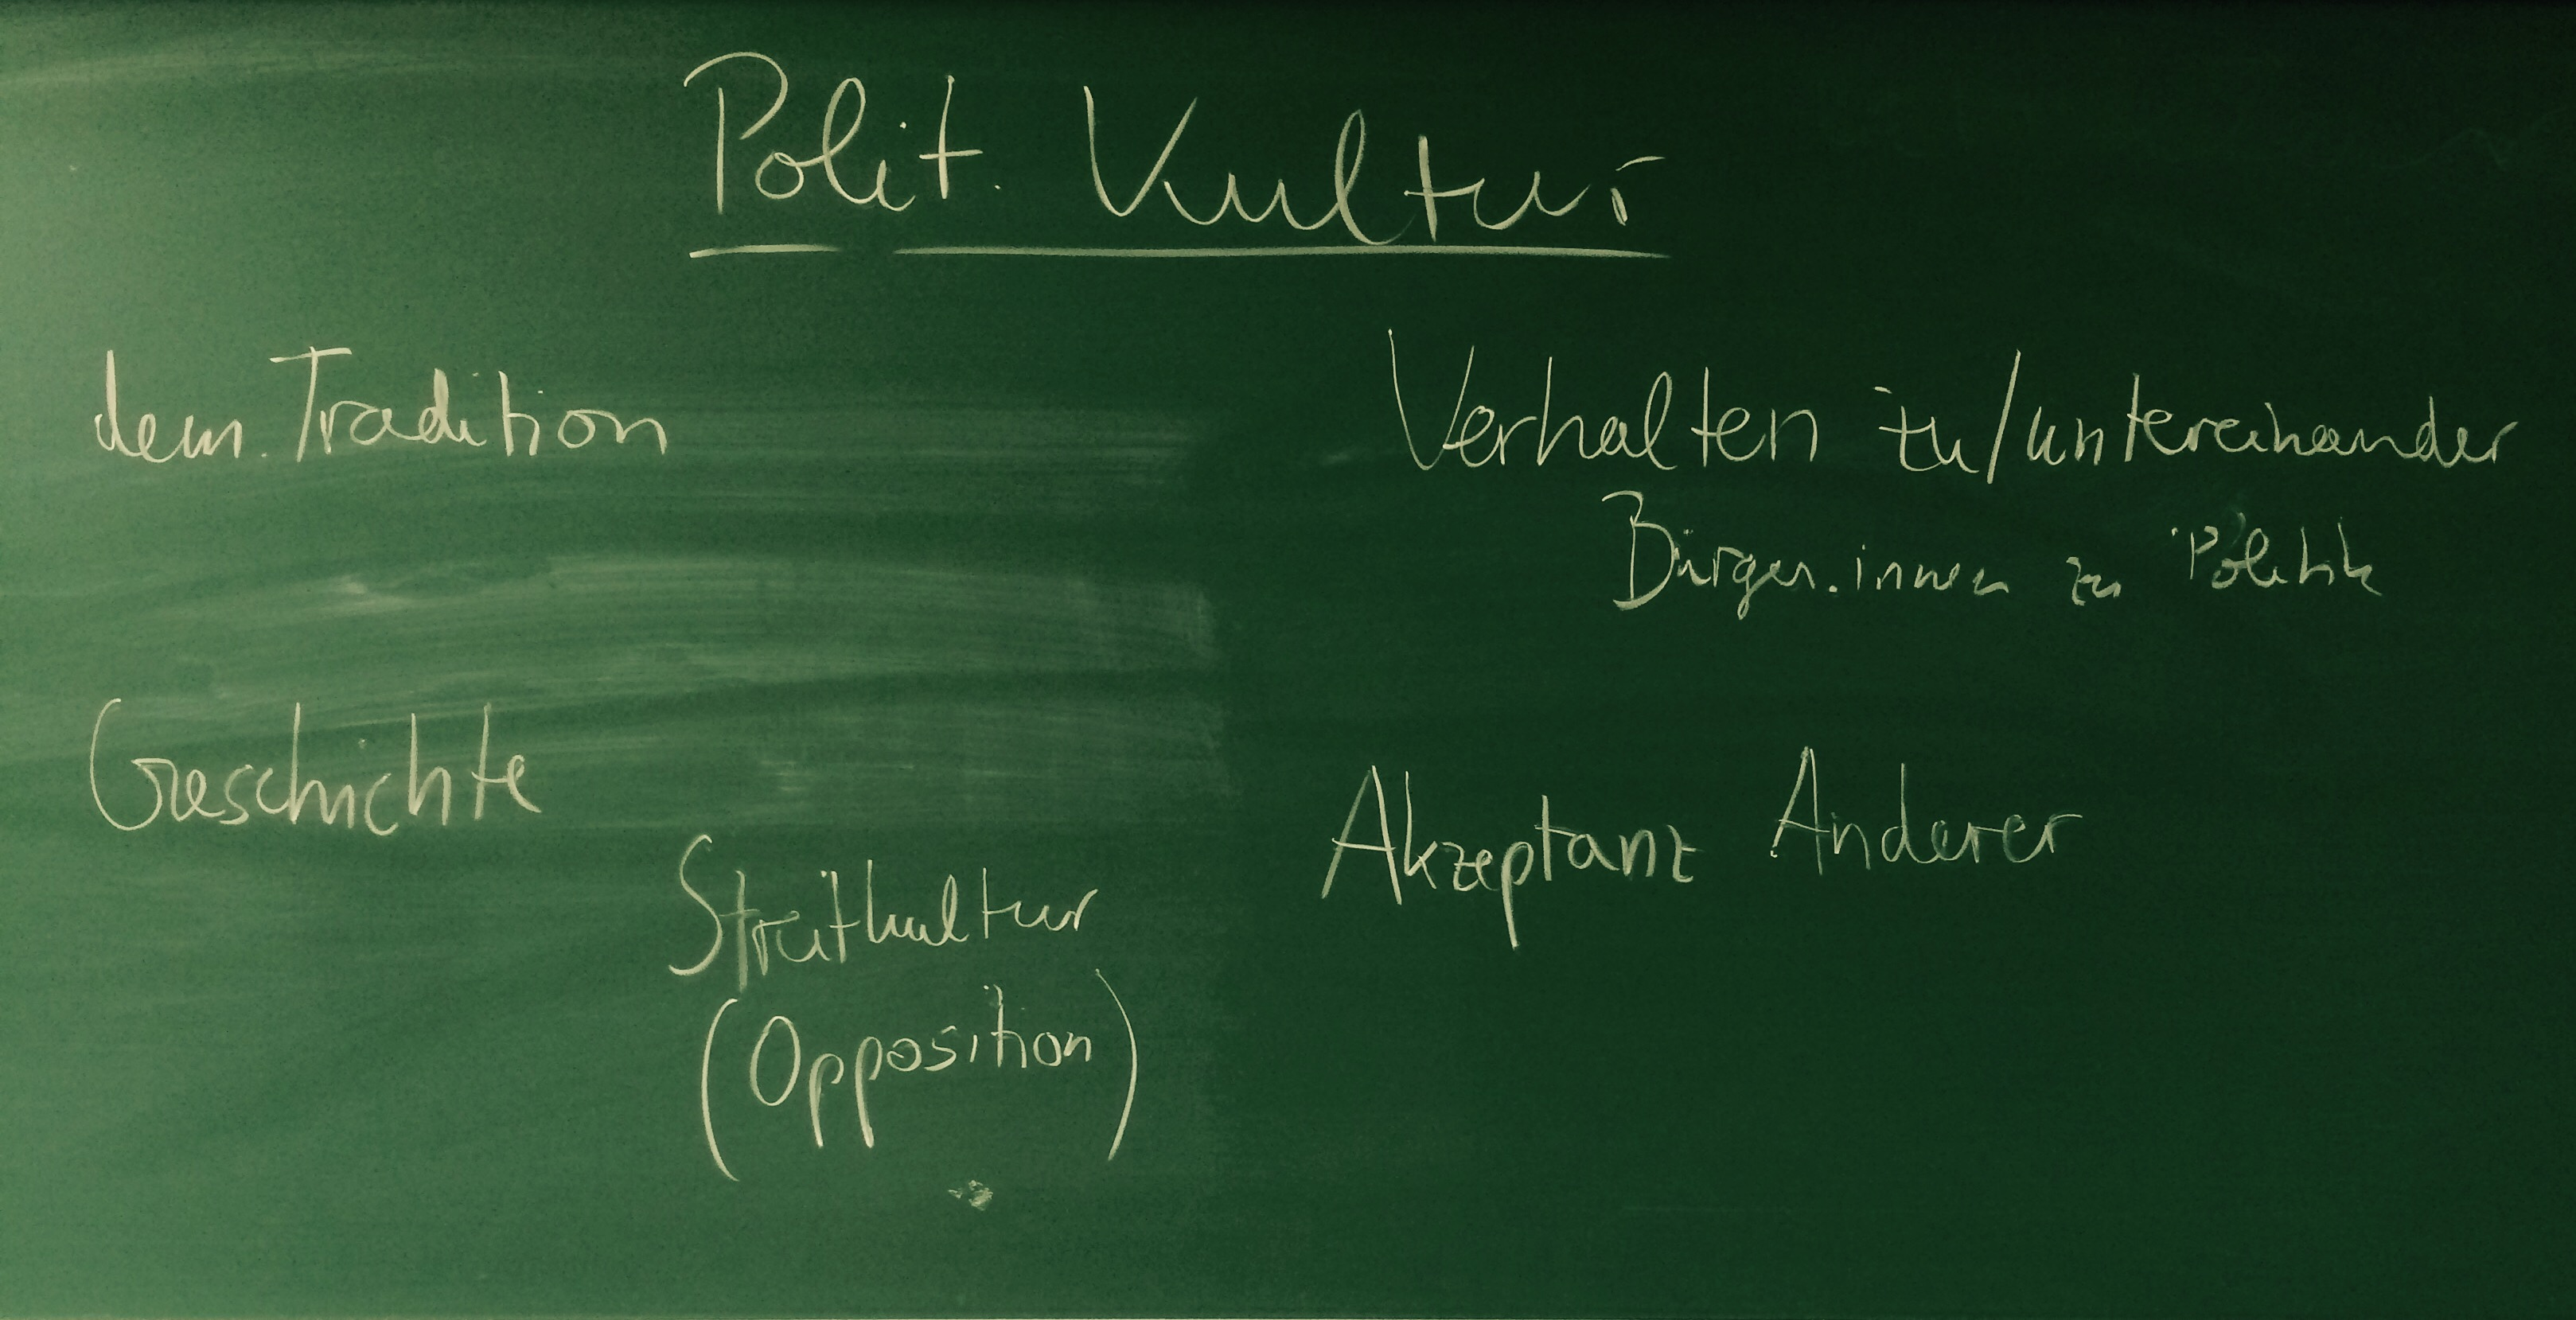
\includegraphics[width=\textwidth]{pics/s3-1.png}
		\caption{\shine{Ideenboard aus einem Seminar}}
	\end{figure}

\end{frame}

\begin{frame}[t]{Politische Kultur}
	\shine{Was ist politische Kultur?} \pause
	\begin{itemize}
		\item „The political culture of a nation is the particular distribution of \textit{patterns of orientation} toward \textit{political objects} among the members of the nation.“ \parencite[14]{Almond1963}	\pause
		\item[$\Rightarrow$] Was ist also Kultur? \pause
		\item[$\Rightarrow$] Auf welcher Analyseebene findet man die polit. Kultur?
	\end{itemize}
\end{frame}

\begin{frame}[t]{Formen der Orientierung}
	\textit{kognitiv} \pause
	\begin{itemize}
		\item \small „(…) that is, knowledge of and belief about the political system, its roles and the incumbents of these roles, ist inputs, and its outputs (…)“ \parencite[15]{Almond1963} \pause
	\end{itemize}
	
	\textit{affektiv} \pause
	\begin{itemize}
		\item\small  „(…) feelings about the political system, its roles, personnel, and performance (…)“ \parencite[15]{Almond1963} \pause
	\end{itemize}
	
	\textit{evaluativ} \pause
	\begin{itemize}
		\item \small „(…) the judgements and opinions about political objects that typically involve the combination of value standards and criteria with information and feeling.“ \parencite[15]{Almond1963} \pause
	\end{itemize}
\end{frame}

\begin{frame}[t]{Formen der Orientierung}
	Welcher Art können diese Orientierungen sein? \pause
	\begin{itemize}
		\item negativ
		\item neutral
		\item positiv
	\end{itemize}
\end{frame}

\begin{frame}[t]{Politische Kultur \& Unterstützung}
	\begin{itemize}
		\item affektiv: diffuse Gefühle \pause
		\item kognitiv: diffuse Ideale, Werte, Normen \pause
		\item evaluativ (I): diffuse und spezifische Bewertungen von Prozessen \pause
		\item evaluativ (II): spezifische Bewertungen von Leistungen
	\end{itemize}

\end{frame}

\begin{frame}[t]{Politische Objekte}
	\shine{4 political objects} \pause
	\begin{itemize}
		\item allgemeine Einstellung gegenüber Aufbau und Struktur des politischen Systems (\textit{system as general object}) \pause
		\item Einstellung gegenüber den Inputmöglichkeiten des politischen Systems (Einschätzung der Teilhabechancen der Bürger) (\textit{input objects}) \pause
		\item Einstellung gegenüber den Outputfähigkeiten des politischen Systems (Bewertung der Ergebnisse der Politik) (\textit{output-objects}) \pause
		\item Selbstwahrnehmung innerhalb des politischen Systems (\textit{self as object})
	\end{itemize}
\end{frame}

\begin{frame}[t]{Zuordnung: Input oder Output?}
	\begin{figure}[ht]
		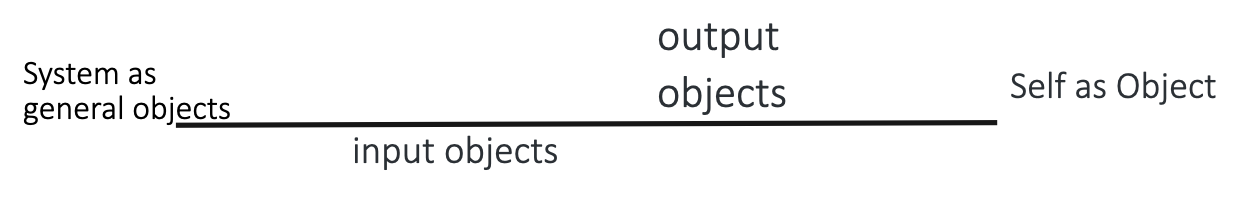
\includegraphics[width=\textwidth]{pics/s3-2.png}
	\end{figure}
	
	\begin{itemize}
		\item Polizei \pause
		\item Gewerkschaften \pause
		\item Parteien \pause
		\item Verwaltung \pause
		\item Gerichte \pause
	\end{itemize}
\end{frame}

\setbeamerfont{itemize/enumerate body}{size = \footnotesize}

\begin{frame}[t]{Politische Kultur: Zusammenfassung}
	\begin{nolist}
		\item[1)] Grundeinheiten der politischen Kultur sind die Einstellungen von Individuen.
		\item[2)] Diese Einstellungen beziehen sich auf politische Objekte.
		\item[3)] Durch eine Aggregation der in einer politischen Einheit (z.B. Nation, Region) vorhandenen individuellen Einstellungen ergibt sich die politische Kultur dieser Einheit.
	\end{nolist}
\end{frame}

\begin{frame}[t]{Politische Kultur: Zusammenfassung}
	\begin{nolist}
		\item[4)] Politische Einstellungen sind ein Individualmerkmal und werden bei Individuen erhoben; die politische Kultur dagegen ist ein Kollektivmerkmal. Als Erhebungseinheit fungieren in der Analyse politischer Kultur somit Individuen; Aussageeinheiten sind Kollektive.
		\item[5)] Das politische Verhalten ist kein Teil der politischen Kultur, sondern bezieht sich auf einen anderen Ausschnitt der politischen Wirklichkeit, der allerdings mit der politischen Kultur verbunden ist.
	\end{nolist}
	
	Quelle: \cite[402]{Gabriel2009}
\end{frame}

\setbeamerfont{itemize/enumerate body}{size = \small}

\begin{frame}[t]{Matrix von Objekten \& Orientierungen}
	\begin{figure}[ht]
		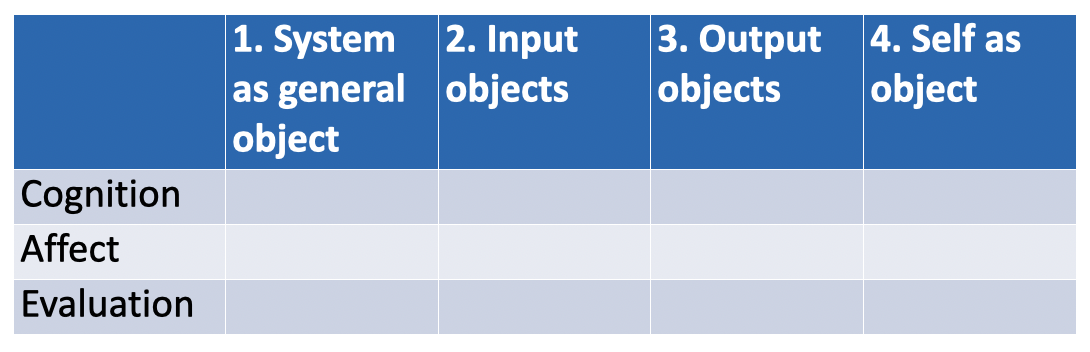
\includegraphics[width=\textwidth]{pics/s3-3.png}
		\caption{Quelle: \cite[16]{Almond1963}}
	\end{figure}

\end{frame}


\begin{frame}[t]{Ergebnisse der Civic Culture Study}
	\begin{figure}[ht]
		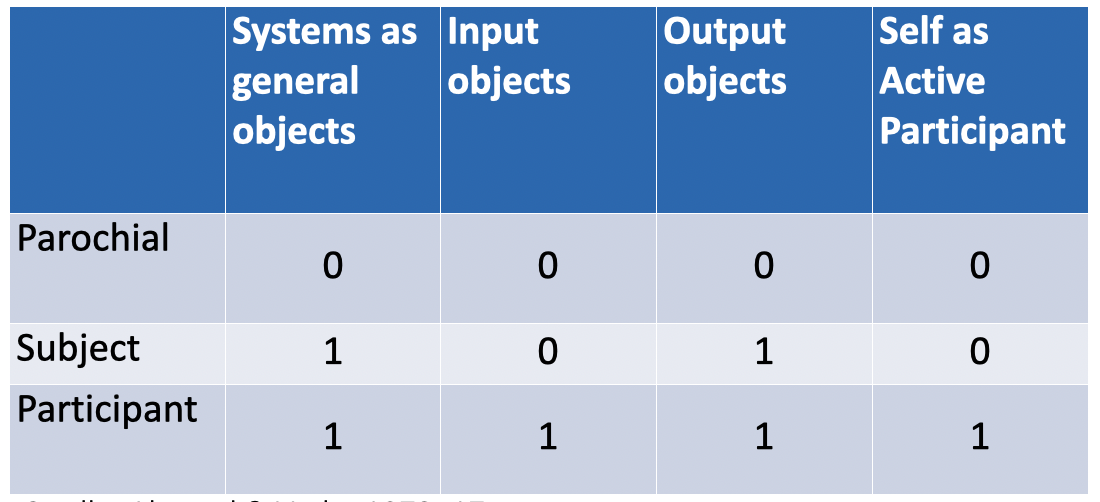
\includegraphics[width=\textwidth]{pics/s3-4.png}
		\caption{Quelle: \cite[17]{Almond1963}}
	\end{figure}

\end{frame}

\begin{frame}[t]{Stabilität des Systems}
	\begin{figure}[ht]
		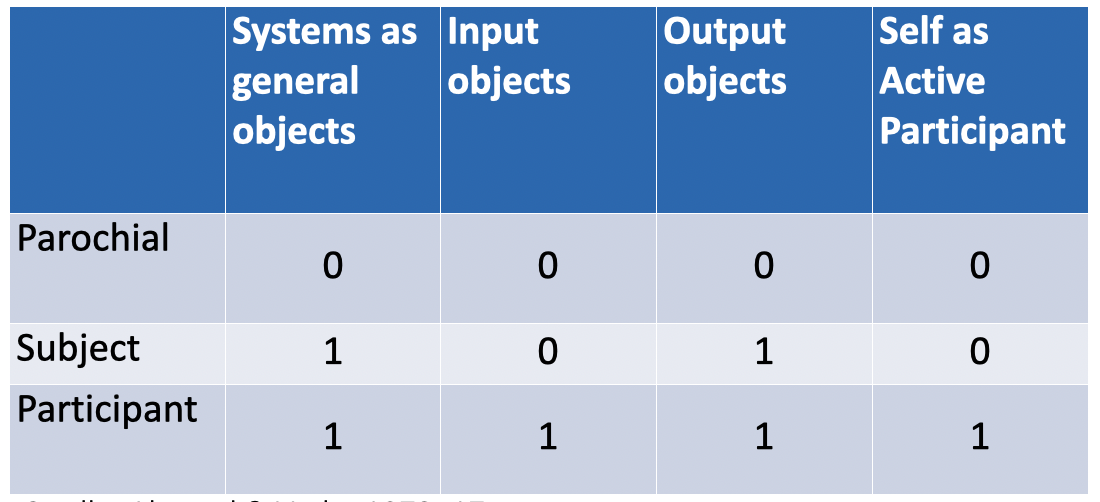
\includegraphics[width=\textwidth]{pics/s3-4.png}
		\caption{Quelle: \cite[22]{Almond1963}}
	\end{figure}

\end{frame}

\begin{frame}[t]{Politische Kultur: Mischtypen}
	\begin{itemize}
		\item Parochial-Subject-Culture
		\item Subject-Participant-Culture
		\item Parochial-Participant-Culture
		\item Civic Culture
	\end{itemize}

\end{frame}

\begin{frame}[t]{Civic Culture}
	\begin{itemize}
		\item „It is a mixture in the first place of parochial, subject and citizen orientations. The orientation of the parochial to primary relationships, the passive political orientation of the subject, the activity of the citizen, all merge within the civic culture.“ \parencite[360]{Almond1980a} \pause
		\item[$\Rightarrow$] balanced set of political orientations
	\end{itemize}

\end{frame}


\begin{frame}[t]{Power \& Responsiveness}
	\shine{Power}
	\begin{itemize}
		\item effektives Regierungshandeln \pause
	\end{itemize}
	
	\shine{Responsiveness}
	\begin{itemize}
		\item Notwendigkeit der Bindung des Handelns an Präferenzen der Bürger:innen
	\end{itemize}
\end{frame}

\begin{frame}[t]{Ergebnisse der Civic Culture Study}
	\begin{itemize}
		\item Studie in fünf Ländern, je 1.000 Befragte
		\item 1959/1960: USA, GB, MEX, IT, DE
		\item  Deutschland hat Untertanenkultur \pause
		\item[$\Rightarrow$] anfällig für Krisen \pause
		\item Bürger informiert, aber passiv und wenig an Politik interessiert
		\item Wahlteilnahme als Pflicht, kein Konzept aktiver Bürgerrolle
		\item Gesellschaft tief gespalten, kaum politische Diskussionen
		\item Politik „schmutzig“, kein Stolz auf neue demokratische Institutionen
	\end{itemize}

\end{frame}

\begin{frame}[t]{Ergebnisse der Civic Culture Study}
	\begin{itemize}
		\item USA und Großbritannien haben Muster einer Civic Culture \pause
		\item[$\Rightarrow$] deshalb der Schluss, dass diese System stabilisiert  \pause
		\item Italien ähnlich wie Deutschland: Subjekt-Kultur
		\item Mexiko: Mischtypus der parochial-partizipativen Kultur \pause
	\end{itemize}

\shine{Folgerungen}
	\begin{itemize}
		\item Politische Kultur in Deutschland und Italien immer noch tradiert von Vorkriegszeit \pause
		\item Untertanenkultur mitverantwortlich für Schwäche / mangelnde Stabilität in Zwischenkriegszeit und Transformation zu Nationalsozialismus
	\end{itemize}
\end{frame}

\begin{frame}{Fragen über Fragen}
	\begin{nolist}
		\item Wie können evaluative von affektiven Orientierungen unterschieden werden?
		\item Wann findet der Erwerb grundlegender Orientierungen statt?
		\item Problem des individualistischen Fehlschlusses
		\item Theoretische Inkonsistenz
		\item Bedeutsamkeit für politische Orientierungen?
		\item Wie lassen sich Orientierungen zum System als Ganzes zusammenfassen? 
		\item Wie genau muss Verteilung aussehen?
	\end{nolist}
\end{frame}

\setbeamerfont{itemize/enumerate body}{size = \footnotesize}

%\begin{frame}[t]{Gruppenarbeit: Praxistest}
%Um empirisch arbeiten zu können, benötigt man immer auch Datensätze. In der Analyse politischer Unterstützung greift man dabei häufig auf regional oder global durchgeführte sozialwissenschaftliche Surveys zurück. \pause
%
%In Kleingruppen wählt ihr einen internationalen oder nationalen Survey aus. Hierzu gibt es dann zwei Aufgaben: 
%\begin{nolist}
%	\item Gewählten Survey selbstständig herunterladen und öffnen
%	\item 3-5 Frageitems heraussuchen und die Verbindung zu den zwei Theorien herstellen \pause
%\end{nolist}
%
%Im Beispiel also z.B. 
%\begin{itemize}
%	\item Frage-Item: „Wie zufrieden sind Sie mit der Leistung der Demokratie in Ihrem Land?“
%	\item[$\Rightarrow$] Theorie-Verbindung: \textit{output}-Bewertung eines Systems (durch Individuen)
%\end{itemize}
%
%\end{frame}
%
%\setbeamerfont{itemize/enumerate body}{size = \small}


\begin{frame}[t]{Assertive Culture}
\begin{itemize}
	\item Überprüfen des Paradigmas durch breiten Forschungsverbund:
	\item \cite{Dalton2014b}: The Civic Culture Transformed. From Allegiant to Assertive Citizens. \pause
	\item[$\Rightarrow$] nicht mehr nur \textit{allegiant culture} über \textit{civic culture} \pause
	\item[$\Rightarrow$] ebenfalls demokratie-stabilisierende \textit{assertive culture} \pause
	\begin{itemize}
		\item[$\Rightarrow$] kritisch gegenüber aktueller Ausformung der Demokratie oder Amtsinhaber:innen 
		\item[$\Rightarrow$] Ruf nach mehr Partzipation
		\item[$\Rightarrow$] aber grundlegende Unterstützung demokratischer Normen/Werte bzw. des demokratischen Systems 
	\end{itemize}
\end{itemize}
\end{frame}

\begin{frame}[t]{Projektidee}
\shine{Ausgangspunkt}: Unterschiedliche Entwicklungen in ehemals staatssozialistischen Ländern der EU (spätestens ab 2010)

\begin{itemize}
	\item Polen, Ungarn (in Teilen Slowakei): Dekonsolidierungstendenzen
	\item Baltikum: weiterhin stabile Demokratie (laut Indizes) \pause
\end{itemize}

\shine{Frage}: Inwieweit geht unterschiedliche Entwicklung in den Staaten einher mit einer unterschiedlichen Entwicklung der politischen Kultur? \pause

\shine{Vorgehensweise}: Vergleich politischer Kultur über Zeit über Länder

\end{frame}

\renewcommand*{\bibfont}{\scriptsize}

\begin{frame}[allowframebreaks]{Literatur}
	\nocite{*}
	\printbibliography[heading = none]
\end{frame}

\section{Mittagspause! \\ Wir treffen uns um 12:30 Uhr wieder.}

\end{document}